\section{Bounded witnesses for reachability}

\ifintuition
\subsection{Intuition}

Our aim is to prove the decidability of the coverability problem for BNRA which can only send a single value in each broadcast. The constructions will actually lead us to a decidability proof for specifications of two different types, both subsuming the coverability specification.

\paragraph*{Step 1 : simplification} In Lemma~\ref{lem:nostar-oneop} we prove that all protocols, even those which can apply several operations when receiving a broadcast, can be simulated by a protocol with a single operation upon reception of a message and no $*$ operation. A previous lemma already allowed us to remove $\diseqtestact$, thus we only have to prove decidability for systems with one operation per reception and only $\enregact$ and $\eqtestact$ operations.

Lemma~\ref{lem:nostar-oneop} is placed at the end of the decidability proof as the constructions defined there may simplify the proof of the lemma (they allow us to prove that BRNA can simulate each other simply by proving that their local runs have the same behaviour).

\paragraph*{Step 2 : run decomposition} Say we have a global run $\rho$ in which an agent broadcasts a message $m_f$. We isolate the local run $u$ of the first agent $a$ broadcasting $m_f$.
In order to execute $u$, we need to receive a sequence of broadcast that matches the sequence of receive transitions in $u$. Let $v$ be a value appearing in $u$.

\begin{itemize}
	\item 
	Say $v$ is not an initial value of $u$, let $w \in \messages^*$ be the sequence of broadcasts received by $a$ with value $v$ in $u$. Then the exact value $v$ does not matter, all $a$ needs is to receive a series of broadcasts with the messages of $w$ all with the same value. This is possible if and only if there exists a global run $\run'$ and a value $v'$ such that $w$ is a subword of the series of broadcasts made in that run with value $v'$. Indeed, if there exists such a run, then $u$ can receive selected broadcasts from $\rho'$ (happening in parallel) in order to get the sequence $w$ of messages with the same value. Conversely, if $u$ receives a sequence $w$ all with the same value in $\rho$, then the prefix of $\rho$ ending just before the broadcast of $m_f$ by $u$ is a fitting candidate for $\rho'$.
	We do not take $\rho$ directly as witness as we want the runs to get shorter as we make the recursive calls.
	
	Here we have our first type of specification, given as a word $w \in \messages^*$. We ask that there exists a global run and a value $v'$ such that $w$ is a subword of the sequence of broadcasts made in the global run with value $v'$.
	
	
	\item 	
	Now suppose $v$ is an initial value of $u$. This situation is very different as other processes need $a$ to send some messages with this value in order to be able to send it back to him.
	The key observation is that once an agent $a'$ other than $a$ has managed to broadcast some message $m$ with value $v$, we have an unlimited supply of such broadcasts:
	Let $w$ be the series of messages broadcast by $a$ with value $v$ before $a'$ makes that broadcast, we now know that there is a global run which, if presented with an external series of broadcasts $w$ with the same value, can then broadcast $m$ with that value.
	We then extend this reasoning and consider the series of broadcast made with value $v$ through $\run$. It can be decomposed as  $(w_0, m_1, w_1, \ldots, m_\ell, w_\ell)$ where $w_0 \cdots w_\ell$ is the sequence of broadcasts made by $a$ with that value and the $m_j$ are placed at the moments where another agent manages for the first time to broadcast that message (from then on we have unlimited supplies of broadcasts with that value and message $m_j$). In particular $\ell \leq \size{\messages}$.
	
	All we have to do is to check for all $j$ that there exists a global run in which some agent broadcasts $m_j$ with a value $v$ that is not one of its initial ones, while having received a series of external broadcasts $w'$ which is of the form $w'_0\cdots w'_{j-1}$ where each $w'_i$ is obtained by adding some letters from $\set{m_0, \ldots, m_i}$ in $w_i$.
	If we have such a run, then with the copycat property we can add an  agent that copies 
	
	This forms our second type of specification, given by a decomposition $(w_0, m_1, w_1, \ldots, m_{j-1}, w_{j-1}, m_j)$, which asks for a run that broadcasts $m_j$ with some value $v'$ which it does not have initially, while receiving a series of  external broadcasts with value $v'$ that match $(w_0, m_1, w_1, \ldots, m_{j-1}, w_{j-1})$.
\end{itemize}   

We can decompose any run satisfying one of those specifications into a local run (the one of the agent having the value initially in the first case, the one of the first agent which manages to broadcast $m_j$ while not having the value initially in the second case) and some number of specifications satisfied by smaller runs.

Hence we can turn a global run satisfying a given specification into a finite tree where nodes are labelled by local runs and specifications of one of the two types above.

\subsection{Bounds on the size of the minimal decomposition}

The previous section provides witnesses for the satisfiability of specifications, in the form of a tree decomposition.

However it is not clear that there is any bound on the size of those trees.

To provide such bounds, we need several observations.
We say that a local run is cheaper than another one if the set of children it spawns in the decomposition tree is easier to achieve: every child of the first run is a subword of a child of the second one.

 First of all we use Lemma~\ref{lem:short-local-runs}, essentially stating that we can reduce any section of a local run of length more than $f(|\prot|)$, where $f$ is a primitive recursive function, to obtain a shorter and cheaper local run.
 This new run may broadcast less messages, thus we cannot say that every local run can be reduced to one of size $f(\size{\prot})$.
 However, we can say that if there exists a local run making some sequence of $N$ broadcasts, then there is one of size at most $Nf(\size{\prot})$, as we can reduce the sections of runs between those broadcasts.
 
 We now define a notion of height of a node, which is not the same as its depth in the tree. Intuitively we put the children of a node $n$ below it if $n$ has to receive messages from them (first case in the previous subsection) and above it if $n$ has to send messages to them (second case).
 The height of the root is $0$, and the height of a child of a node $n$  is  the one of $n$ minus one if it is of the first type of specification, plus one otherwise.
 
 Nodes of minimal height (except maybe the root) are nodes of the second type which only have children of the first type, hence all they have to do is broadcast one single message (given by their father). Hence their length is at most $f(\size{\prot})$. 
 
 Now assume we have a bound $M$ on runs of height $h$. A run of height $h-1$ sees at most $r$ different initial values. Hence it has at most $\size{\messages}r$ children of the second type, and for each corresponding specification it has to make at most $M$ broadcasts, as each of those children makes at most $M$ receiving actions.
 Moreover, if it is of the first type, it also has to provide broadcasts for its father, but again his father has height $h$, thus will require at most $M$ broadcasts.
 
 Overall a local run at height $h-1$ needs to make a series of at most $M(\size{\messages} r +1)$ broadcasts. If that can be done, it can be done by a local run of length at most $[M(\size{\messages} r +1)](f(\size{\prot})+1)$.
 
 As a result, we can bound the size of a node of height $h$ by $g(\size{\prot}, hmax-h)$, where $hmax$ is the maximal height of the tree and $g$ is a primitive recursive function.
 
 This allows us to bound $hmax$: indeed consider the branch reaching the highest point in the tree. Along that branch we can extract a sequence of nodes of the second type $\mu_0, \ldots, \mu_{hmax}$ such that $\mu_i$ has height $i$ for all $i$. If there are some $i<j$ such that $\mu_i$ and $\mu_j$ produce the same broadcast but $\mu_j$ is cheaper then we can reduce the branch.
 The bounds on the lengths of the $\mu_i$ and the latter property allow us to bound $hmax$ with a function from the class $F_{\omega^\omega}$ (see, for instance, \cite{SchmitzS2011upperHigman}).
 
 This also gives us a bound on the size of the root (which is also in $F_{\omega^\omega}$). From there we bound the minimal height of a node of this tree. The argument is that in order to reach a minimal height $hmin$ with a branch, we need to have along that branch a subsequence of nodes of the first type $\mu_0, \ldots, \mu_{-hmin}$ such that $\mu_i$ has height $-i$. If there exist $i<j$ such that $\mu_i$ broadcasts a subword of $\mu_j$ we can reduce the branch. Otherwise, the same results on bad sequences of words  for the subword order allow us to bound the minimal height of a node in that tree with a function of $F_{\omega^\omega}$.
 As both the minimal and maximal heights in the tree are bounded by such functions, the size of a node of that tree is also bounded by such a function (using the bound on nodes based on their height). This is also a bound on the branching of the tree, as the number of children of a node is bounded by the number of values seen in its local run, thus by the size of that run.
 
 The number of different nodes along a branch is also bounded, hence also the size of that branch (if the same node appears twice we can reduce the branch).
 This lets us bound the overall size of the tree with a function of $F_{\omega^\omega}$, yielding decidability and complexity of the problem.

\subsection{Formal proof}
\fi


\textbf{For now we assume that the BRNA do not contain $*$ operations and apply only one operation for each message received. The general case reduces to this one (lemma \ref{lem:simple-reduction}).}

\begin{definition}
	A ""local configuration"" is a pair $(q, \nu) \in Q \times ([1,r] \to \nats)$.
	A ""local run"" is a sequence of local transitions $(q_0, \nu_0) \xrightarrow{op_1} (q_1, \nu_1) \xrightarrow{op_2} \cdots \xrightarrow{op_k} (q_k, \nu_k)$ with $op_1, \ldots, op_k \in Op_r^\messages$.
	
	Given a value $v \in \nats$, the $v$-input of a local run $u$, which we denote by $\vinput{v}{u}$, is the sequence of messages received through $u$ with value $v$.
	Its $v$-output, which we denote by $\voutput{v}{u}$, is the sequence of messages of broadcasts made in $u$ with value $v$. 
	Its $v$-vision, which we denote by $\vision{v}{u}$, is the sequence of messages of broadcasts made or received in $u$ with value $v$.
	
	The ""input"" of $u$ is the set $\Input{u} = \set{\vinput{v}{u} \mid v \in \nats}$.
	Its ""output"" is the set $\Output{u}=\set{\voutput{v}{u} \mid v \in \nats}$.
	Its ""trace"" $\trace{u} \in Op^\messages_r$ is the sequence of operations executed by $u$.
	
	We define a preorder on such sets of words:
	Given $W, W' \in \powerset{\Sigma^*}$, $W \unlhd W'$ if $W \subseteq W'\downarrow$, where $W'\downarrow$ stands for the set of subwords of words in $W'$.
\end{definition}



\begin{definition}
	Let $m_1, \cdots, m_\ell \in \messages$, $w_0, \ldots, w_\ell \in \messages^*$, we say that a word $w \in \messages^*$ ""decomposes as"" $(w_0, m_1, \ldots, m_\ell, w_\ell)$ if $w = w'_0 w'_1 \cdots w'_\ell$ where for all $j$, $w'_j$ can be obtained from $w_j$ by adding some letters from $\set{m_1, \ldots, m_{j-1}}$.
	
	An unfolding of $(w_0, m_1, \ldots, m_\ell, w_\ell)$ is a subword of a word that decomposes as $(w_0, m_1, \ldots, m_\ell, w_\ell)$. 
	
	We define a preorder on decompositions:
	$(w_0, m_1, \ldots, m_\ell, w_\ell) \preceq (w'_0, m'_1, \ldots, m'_k, w'_k)$ if the set of unfoldings of $(w_0, m_1, \ldots, m_\ell, w_\ell)$ is included in the one of $(w'_0, m'_1, \ldots, m'_k, w'_k)$
\end{definition}


\begin{definition}
	A ""tree decomposition""  is
	a finite tree where each node has two labels:
	\begin{itemize}
		\item The first one is a local run of $\prot$. 
		
		\item The second one is a ""specification"", which is either a word $w \in \messages^*$ (we say that the node is a ""boss node"") or a decomposition along with a message $(w_0, m_1, \ldots, w_\ell), m$ (""follower node""). 
	\end{itemize} 
	
	It must satisfy the following conditions:
	Let $\mu$ be a node of that tree, and $u$ the local run labelling it.
	
	If it is a "boss node" labelled by some word $w \in \messages^*$ then there must exist $v \in \nats$ an initial value of $u$ such that
	\begin{itemize}
		\item $w$ "decomposes as" $(w_0, m_1, w_1, \ldots, m_\ell, w_\ell)$ with $w_0 \cdots w_\ell$ the $v$-input of $u$, and for all $1 \leq j \leq \ell$, $\mu$ has a child which is an "follower node" labelled $(w_0, m_1, w_1, \ldots, m_{j-1}, w_{j-1}), m_j$.
		
		\item For all $v' \neq v$ appearing in $u$,
		\begin{itemize}
			\item If $v'$ is an initial value of $u$ then the $v'$-vision of $u$ "decomposes as"  $(w'_0, m'_1, w'_1, \ldots, m'_k, w'_k)$ where $w'_0 w'_1 \ldots w'_k$ is the $v'$-output of $u$ and for all $1 \leq j \leq k$ $\mu$ has a child which is an "follower node" labelled $(w_0, m_1, w_1, \ldots, m_{j-1}, w_{j-1}), m_j$.  
			
			\item If $v'$ is not an initial value then $\mu$ has a child which is a "boss node" labelled by $w'$ the $v'$-input of $u$.
		\end{itemize}
	\end{itemize}
	
	If it is an "follower node" labelled by some $(w_0, m_1, w_1, \ldots, m_\ell, w_\ell), m$ then there must exist $v \in \nats$ an initial value of $u$ such that
	\begin{itemize}
		\item $u$ ends with a broadcast of $m$ with value $v$.
		
		\item The $v$-input of $u$ is a subword of some $w' = w'_0\cdots w'_\ell$ where, for all $j$, $w'_j$ can be obtained by adding some $m_1, \ldots, m_{j}$ to $w_j$.
		
		\item For all $v' \neq v$ appearing in $u$,
		\begin{itemize}
			\item If $v'$ is an initial value of $u$ then the $v'$-vision of $u$ "decomposes as"  $(w'_0, m'_1, w'_1, \ldots, m'_k, w'_k)$ where $w'_0 w'_1 \ldots w'_k$ is the $v'$-output of $u$ and for all $1 \leq j \leq k$ $\mu$ has a child which is an "follower node" labelled $(w_0, m_1, w_1, \ldots, m_{j-1}, w_{j-1}), m_j$.  
			
			\item If $v'$ is not an initial value then $\mu$ has a child which is a "boss node" labelled by $w'$ the $v'$-input of $u$.
		\end{itemize}
	\end{itemize}
\end{definition}


% Old definition

%\begin{definition}
%	We define two types of specifications for runs of a given "protocol" $\prot$:
%	
%	\begin{itemize}
%		\item The first one is the ""boss type"", and is given by a word $w$ over $\messages$. There should exist some value $v \in \nats$ such that the $v$-output of the run has $w$ as a subword.
%		
%		\item The second one is the ""follower type"". It is given by sequences of letters $m_1, \ldots, m_\ell \in \messages$ and words $w_0, \ldots, w_\ell$ over $\messages$, and a letter $m \in \messages$, such that all $m_j$ are distinct from $m$ and from each other.
%		There should exist some value $v$ such that the run takes as input a word $w'$ that "decomposes as" $(w_0, m_1, \ldots, m_\ell, w_\ell)$, and whose $v$-output contains an $m$.
%	\end{itemize}
%\end{definition}

%\begin{definition}
%	A ""tree decomposition"" of a run $\run$ with respect to a "specification" is
%	a tree whose nodes are labelled by local runs $u$ of $\prot$ and either by "boss specifications" $w$ ("boss nodes") or by "follower specifications" $(w_0, m_1, w_1, \ldots, m_\ell, w_\ell, m)$ ("follower nodes"). 
%	
%	It must satisfy the following conditions:
%	Let $\mu$ be a node of that tree, and $u$ the local run labelling it.
%	
%	If it is a "boss node" labelled by some $w$ then there must exist $v \in \nats$ an initial value of $u$ such that
%	\begin{itemize}
%		\item $w$ "decomposes as" $(w_0, m_1, w_1, \ldots, m_\ell, w_\ell)$ with $w_0 \cdots w_\ell$ the $v$-input of $u$, and for all $1 \leq j \leq \ell$ $\mu$ has a child which is an "follower node" labelled $(w_0, m_1, w_1, \ldots, m_{j-1}, w_{j-1}), m_j$.
%		
%		\item For all $v' \neq v$ appearing in $u$,
%		\begin{itemize}
%		\item If $v'$ is an initial value of $u$ then the $v'$-vision of $u$ "decomposes as"  $(w'_0, m'_1, w'_1, \ldots, m'_k, w'_k)$ where $w'_0 w'_1 \ldots w'_k$ is the $v'$-output of $u$ and for all $1 \leq j \leq k$ $\mu$ has a child which is an "follower node" labelled $(w_0, m_1, w_1, \ldots, m_{j-1}, w_{j-1}), m_j$.  
%			
%		\item If $v'$ is not an initial value then $\mu$ has a child which is a "boss node" labelled by $w'$ the $v'$-input of $u$.
%		\end{itemize}
%	\end{itemize}
%
%	If it is an "follower node" labelled by some $(w_0, m_1, w_1, \ldots, m_\ell, w_\ell, m)$ then there must exist $v \in \nats$ an initial value of $u$ such that
%	\begin{itemize}
%		\item $u$ ends with a broadcast of $m$ with value $v$.
%		
%		\item The $v$-input of $u$ is a subword of some $w' = w'_0\cdots w'_\ell$ where, for all $j$, $w'_j$ can be obtained by adding some $m_1, \ldots, m_{j}$ to $w_j$.
%		
%		\item For all $v' \neq v$ appearing in $u$,
%		\begin{itemize}
%			\item If $v'$ is an initial value of $u$ then the $v'$-vision of $u$ "decomposes as"  $(w'_0, m'_1, w'_1, \ldots, m'_k, w'_k)$ where $w'_0 w'_1 \ldots w'_k$ is the $v'$-output of $u$ and for all $1 \leq j \leq k$ $\mu$ has a child which is an "follower node" labelled $(w_0, m_1, w_1, \ldots, m_{j-1}, w_{j-1}), m_j$.  
%			
%			\item If $v'$ is not an initial value then $\mu$ has a child which is a "boss node" labelled by $w'$ the $v'$-input of $u$.
%		\end{itemize}
%	\end{itemize}
%\end{definition}

\begin{definition}
	A "tree decomposition" satisfies a specification $w$ if its root is a "boss node" and $w$ is a subword of its specification label.
	A "tree decomposition" satisfies a follower specification $(w_0, m_1, w_1, \ldots, m_k, w_k) ,m$ if its root is an "follower node" labelled with a "decomposition" $(w'_0, m'_1, w'_1, \ldots, m'_\ell, w'_\ell,m)$ such that  $(w_0, m_1, w_1, \ldots, m_k, w_k) \preceq (w'_0, m'_1, w'_1, \ldots, m'_\ell, w'_\ell)$.
	\cortoin{To adapt (maybe)}
\end{definition}

We will now prove that there exists a finite run satisfying a specification if and only if there exists a finite tree satisfying that same specification.
We first decompose a run into a tree, then we build a run from a tree. Note that by applying consecutively these two transformations we obtain in general a much larger run than the initial one. That is because each node of the tree is associated with a part played in the run by some agent. In the initial run, the same agent may play many different parts, while in the run we construct from the tree we use different agents for each node of the tree.

Also note that the interpretation of the "follower nodes" changes between the two directions: When building the tree an follower node labelled $(w_0, m_1, w_1, \ldots, m_k, w_k) ,m$ means that there exists a global run in which some agent receives a sequence of messages which decomposes as  $(w_0, m_1, w_1, \ldots, m_k, w_k)$ before broadcasting $m$, all with a value $v$ that is not one of its initial ones.

When building the run an follower node means that there exists a global run which receives a series of external broadcasts which decomposes as $(w_0, m_1, w_1, \ldots, m_k, w_k)$, with a value $v$ that it initially does not contain, and eventually broadcasts $m$ with that value.

\begin{lemma}
	If there exists a finite run $\rho$ satisfying some "specification" then there exists a finite "tree decomposition" satisfying that "specification".
\end{lemma}

\begin{proof}
	We proceed by strong induction on the length of $\rho$.
	Let $N \in \nats$, suppose the lemma holds for all runs of length less than $N$.
	
	\textbf{Case 1: The specification is a "boss specification"}
	
	Let $\run$ be a run of length $N$ satisfying a "boss specification" $w$.
	There exists a value $v$ such that $w$ is a subword of the sequence of messages broadcast with value $v$ through $\run$. Let $w'$ be the latter sequence.
	If $w$ is empty then the tree decomposition with one node labelled with the an empty local run and $w$ satisfies $w$.	
	Otherwise let $a$ be the agent which has $v$ as an initial value, let $u$ be its local run in $\run$. 
	We decompose $w'$ as $(w'_0, m_1, w'_1, \ldots, m_\ell, w'_\ell)$, where $w'_0\cdots w'_\ell$ is the sequence of messages broadcast by $a$ with value $v$, and the $(m_j)_{1\leq j\leq \ell}$ are the elements of $\messages$, placed at the times at which they are first broadcast by an agents other than $a$ with value $v$. If there is no such broadcast of a message $m$, then it does not appear as an $m_j$. This is clearly a "decomposition" of $w'$.
	
	For all $1 \leq j \leq \ell$, there exists a prefix of 
\end{proof}

\begin{lemma}
	If there exists a finite "tree decomposition" whose root is labelled with some "specification" then there exists  a finite run $\rho$ satisfying that specification.
\end{lemma}

\begin{proof}
	\cortoin{TODO}
\end{proof}

\begin{lemma}
	If two protocols $\prot, \prot'$ are such that for all local run $u$ of one of them, the other has a local run with the same inputs and outputs, then they satisfy the same queries. 
\end{lemma}

\begin{proof}
	\cortoin{TODO}
\end{proof}



\begin{lemma}
	\label{lem:simple-reduction}
	For all "protocol" $\prot$ there is a "simple protocol" $\prot'$ with one more register satisfying the same queries.
\end{lemma}

\begin{proof}
	\cortoin{Ancienne preuve, à adapter ou réécrire}
	
	We construct $\prot'$ as follows: It has one more register than $\prot$, but stores in its state the current state of $\prot$ and a mapping $map : [1,r] \to [1,r+1]$ from registers of $\prot$ to its own registers.
	
	Intuitively, it is going to use its registers to store the different values that are in the registers of $\prot$, and the mapping to keep track of which registers contain which values.
	When a value is received it guesses whether it is one of the existing values or a fresh one, and updates the registers and the mapping accordingly.
	The extra register of $\prot'$ is not necessary, but simplifies the proof.
	
	Formally, we set $\prot = (Q, \messages, \Delta, q_0)$. The set of states of $\prot'$ is $Q \times ([1,r] \to [1,r])$. 
	There is a transition $(q, map) \xrightarrow{\br{m}{i}} (q', map')$ if and only if $map = map'$ and $\prot$ has a transition $q \xrightarrow{\br{m}{j}} q'$ with $map(j) = i$.
	
	There is a transition $(q, map) \xrightarrow{\rec{m}{j}{\enregact}} (q', map')$ if and only if there is a transition $q \xrightarrow{\recmulti{m}{op_1\cdots op_r}} q'$ in $\prot$ such that $op_i \neq \eqtestact$ for all $i$ and $map^{-1}(j) =\emptyset$ and for all $i \in [1,r]$, $map'(i) = map(i)$ if $op_i = *$ and $map'(i) = j$ if $op_i = \enregact$.
	
	There is a transition $(q, map) \xrightarrow{\rec{m}{j}{\eqtestact}} (q', map')$ if and only if there is a transition $q \xrightarrow{\recmulti{m}{op_1\cdots op_r}} q'$ in $\prot$ such that for all $i\in [1,r]$,
	\begin{itemize}
		\item If $op_i = \eqtestact$ then $map(i) = map'(i) = j$
		
		\item If $op_i = \enregact$ then $map'(i) = j$
		
		\item If $op_i = *$ then $map'(i)= map(i)$
	\end{itemize}
	
	
	We prove by induction on $\size{u}$ that for all "local run" $u$ of $\prot$ there exists a "local run" $u'$ of $\prot'$ with the same "trace" and such that if the last configuration of $u$ is $(q,f)$ and the last configuration of $u'$ is $((q',map), f')$ then $q=q'$ and for all $i$, $f(i) = f'(map(i))$.  
	
	\cortoin{TODO}
	
	We prove by induction on $\size{u'}$ that for all "local run" $u'$ of $\prot'$ there exists a "local run" $u$ of $\prot$ with the same "trace" and such that if the last configuration of $u$ is $(q,f)$ and the last configuration of $u'$ is $((q',map), f')$ then $q=q'$ and for all $i$, $f(i) = f'(map(i))$.
	
	\cortoin{TODO}  
\end{proof}

\begin{lemma}
	Let $w$ be a "boss specification".
	Let $\tau$ be a "tree decomposition" whose root is labelled with $w$.
	Let $\mu, \mu'$ be two "boss nodes" of $\tau$, $u, v$ and $u', v'$ the associated local runs.
	If $\mu$ is an ancestor of $\mu'$ and the $v$-output of $\mu$ is a subword of the $v'$-output of $\mu'$ then there exists a smaller "tree decomposition" with its root labelled $w$.  
\end{lemma}

\begin{proof}
	\cortoin{TODO}
\end{proof}

\begin{lemma}
	Let $w$ be a "boss specification".
	Let $\tau$ be a "tree decomposition" whose root is labelled with $w$.
	Let $\mu, \mu'$ be two "follower nodes" of $\tau$, $u, v$ and $u', v'$ the associated local runs.
	If $\mu$ is an ancestor of $\mu'$ and the $v'$-input of $\mu'$ is a subword of the $v$-input of $\mu$ and their required output message is the same then there exists a smaller "tree decomposition" with its root labelled $w$.  
\end{lemma}

\begin{proof}
	\cortoin{TODO}
\end{proof}

\begin{lemma}
	Let $u_1$, $u_2$ be two local runs of a protocol $\prot$ with the same sequence of transitions, $(q_1, \nu_1)$ the first local configuration of $u_1$, $(q_2, \nu_2)$ the last one of $u_2$. Then there i a local run $u$ with the same sequence of transitions as $u_1$ and $u_2$ from $(q_1, \nu_1)$ to $(q_2, \nu_2)$. 
\end{lemma}

\begin{figure}
	

	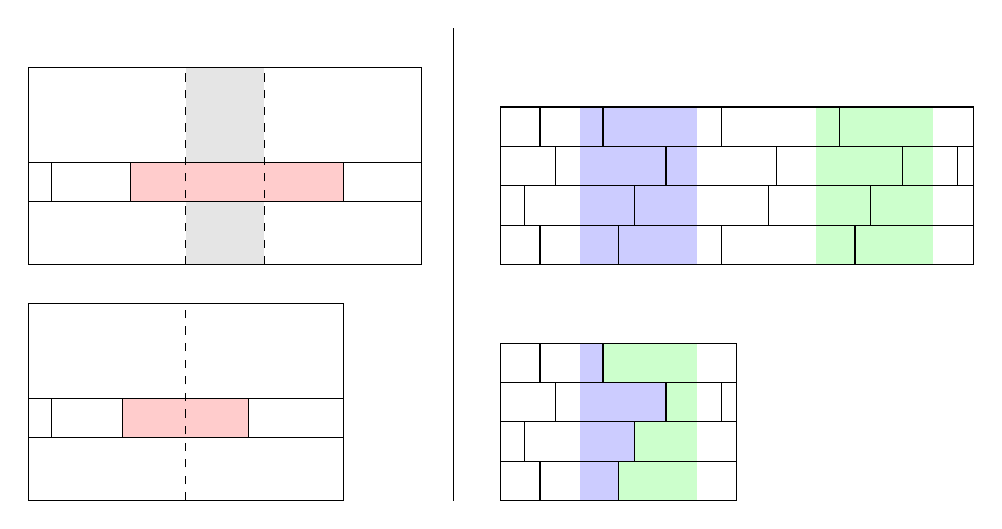
\begin{tikzpicture}
		\draw[white,fill=gray!20] (2,0) rectangle (3,0.8);
		\draw[white,fill=gray!20] (2,1.3) rectangle (3,2.5);
		
		\draw (0,0) rectangle (5,2.5);
		
		\draw (0,0.8) rectangle (5,1.3);
		
		\draw (0,0.8) rectangle (0.3,1.3);
		\draw (0,0.8) rectangle (1.3,1.3);
		\draw[fill=red!20] (1.3,0.8) rectangle (4,1.3);
		
		\draw[dashed] (2,0) -- (2,2.5);
		\draw[dashed] (3,0) -- (3,2.5);
		
		
		
		\draw (0,-3) rectangle (4,-0.5);
		
		\draw (0,-2.2) rectangle (4,-1.7);
		
		\draw (0,-2.2) rectangle (0.3,-1.7);
		\draw (0.3,-2.2) rectangle (1.3,-1.7);
		\draw[fill=red!20] (1.2,-2.2) rectangle (2.8,-1.7);
		
		\draw[dashed] (2,-3) -- (2,-0.5);
		
		\draw (5.4,-3) -- (5.4,3);
		
		
		\draw[white,fill=blue!20] (7,0) rectangle (8.5,2);
		\draw[white,fill=green!20] (10,0) rectangle (11.5,2);
		
		\draw (6,0) rectangle (12,2);
		
		\draw (6,0) rectangle (12,0.5);
		\draw (6,0) rectangle (12,1);
		\draw (6,0) rectangle (12,1.5);
		
		\draw (6,0) rectangle (6.5,0.5);
		\draw (6,0) rectangle (7.5,0.5);
		\draw (6,0) rectangle (8.8,0.5);
		\draw (6,0) rectangle (10.5,0.5);
		
		\draw (6,0.5) rectangle (6.3,1);
		\draw (6,0.5) rectangle (7.7,1);
		\draw (6,0.5) rectangle (9.4,1);
		\draw (6,0.5) rectangle (10.7,1);
		
		\draw (6,1) rectangle (6.7,1.5);
		\draw (6,1) rectangle (8.1,1.5);
		\draw (6,1) rectangle (9.5,1.5);
		\draw (6,1) rectangle (11.1,1.5);
		\draw (6,1) rectangle (11.8,1.5);
		
		\draw (6,1.5) rectangle (6.5,2);
		\draw (6,1.5) rectangle (7.3,2);
		\draw (6,1.5) rectangle (8.8,2);
		\draw (6,1.5) rectangle (10.3,2);
		
		
		\draw[white, fill=blue!20] (7,-3) rectangle (7.5,-2.5);
		\draw[white,fill=blue!20] (7,-2.5) rectangle (7.7,-2);
		\draw[white,fill=blue!20] (7,-2) rectangle (8.1,-1.5);
		\draw[white,fill=blue!20] (7,-1.5) rectangle (7.3,-1);
		
		\draw[white,fill=green!20] (7.5,-3) rectangle (8.5,-2.5);
		\draw[white,fill=green!20] (7.7,-2.5) rectangle (8.5,-2);
		\draw[white,fill=green!20] (8.1,-2) rectangle (8.5,-1.5);
		\draw[white,fill=green!20] (7.3,-1.5) rectangle (8.5,-1);
		
		
		
		\draw (6,-3) rectangle (9,-2.5);
		\draw (6,-3) rectangle (9,-2);
		\draw (6,-3) rectangle (9,-1.5);
		\draw (6,-3) rectangle (9,-1);
		
		\draw (6,-3) rectangle (6.5,-2.5);
		\draw (6,-3) rectangle (7.5,-2.5);
		
		\draw (6,-2.5) rectangle (6.3,-2);
		\draw (6,-2.5) rectangle (7.7,-2);
		
		\draw (6,-2) rectangle (6.7,-1.5);
		\draw (6,-2) rectangle (8.1,-1.5);
		\draw (6,-2) rectangle (8.8,-1.5);
		
		\draw (6,-1.5) rectangle (6.5,-1);
		\draw (6,-1.5) rectangle (7.3,-1);
		
	\end{tikzpicture}


	\caption{Illustration of the proof of Lemma~\ref{lem:short-local-runs}. Lines correspond to registers, and vertical separations are times at which the value of that register changes. If one register $i$ keeps the same value for a long enough time (on the left), we apply the induction hypothesis to shorten the projection of the run on the other registers. As the value of $i$ does not change, the resulting run is still valid. If all registers change values often (on the right), then if the run is long enough we can find two identical sequences of transitions during which all values are renewed. We can then obtain a shorter run by glueing them together as in the picture.}
\end{figure}

\cortoin{The tower bound of Lemma~\ref{lem:short-local-runs} is tight, in the sense that some local runs may need to have length a tower of exponentials of height the number of registers.}

\cortoin{The tower bound of Lemma~\ref{lem:short-local-runs} also holds for pushdown automata, and for all transition systems which have some kind of pumping lemma.}


\begin{lemma}
	\label{lem:short-local-runs}
	Let $\prot$ be a protocol with $r$ registers.
	Let $u$ be a "local run" of $\prot$ with an "input" $I$.
	Let $u_1, u_2, u_3$ be such that $u=u_1u_2u_3$.
	If $\size{u_2} > TOWER$, then there exists $u'_2$ such that $u_1u'_2u_3$ is a local run of $\prot$ with smaller "input" than $u$. 
\end{lemma}

\begin{proof}
	The statement of this lemma is adapted to ease its use in the other proofs.
	In order to prove it, we show a stronger statement.	
	For this proof we will allow our protocols to execute local actions from a finite alphabet $\Sigma$, which are not associated with any broadcast or receive operation.	
	
	We will show the following result, which directly implies the lemma:
	Let $\prot$ be a protocol with $r$ registers, let $u$ be a "local run" of $\prot$ from "local configuration" $(q_0, \nu_0)$ to $(q_{end}, \nu_{end})$ with an input $I$. If $\size{u} \geq TOWER$, then there exists a shorter local run $u'$ from $(q_0, \nu_0)$ to $(q_{end}, \nu_{end})$, with a smaller "input" and such that the sequence of local actions in $u'$ is a subword of the one in $u$.
	We proceed by induction on $r$.
	
	If $r=0$ then if $\size{u} > TOWER = \size{Q}$ then $u$ visits twice the same state, hence the same local configuration as there are no registers, and the sequence between those two moments can be deleted, yielding the result.
	
	Let $r>0$, suppose the proposition holds for $r-1$.
	Let $u$ be a run of $\prot$, a protocol with $r$ registers, with $\size{u} > TOWER$.
	
	\begin{itemize}
		\item If there exists $i \in [1,r]$ such that $u$ has a factor $u_f$ in which the value of register $i$ does not change and with $\size{u_f} > TOWER$, then let $\Tilde{\prot}$ be $\prot$ where every operation $op$ over $i$ has been replaced with a local action $a_{op}$. Note that $\Tilde{\prot}$ only uses $r-1$ registers. 
		Let $\Tilde{u_f}$ be the run following $u_f$ in $\prot$, where every transition $q \xrightarrow{op} q'$ with an operation on $i$ has been replaced with $q \xrightarrow{a_{op}} q'$.
		
		By induction hypothesis we have that there exists $\Tilde{u'_f}$ shorter than $\Tilde{u_f}$, with the same start and end local configurations, a smaller input, and a sequence of local actions that is a subword of the one of $\Tilde{u_f}$.
		
		We conclude that the corresponding sequence of transitions $u_f'$ in $\prot$ is a local run with the same initial and final local configurations as $u_f$, as the value of register $i$ stays the same throughout both runs. .
		
		\item If no register keeps the same value for more than $TOWER$ steps, then any run $u$ of length at least $M_{r-1} ((\size{\Delta})^{M_{r-1}} +1)$ can be split into $(\size{\Delta})^{M_{r-1}} +1$ segments of size $M_{r-1}$. There are $\size{\Delta}^{M_{r-1}}$ different sequences of transitions, thus by the pigeonhole principle we have $u = \pi_1 \sigma_1 \pi_2 \sigma_2 \pi_3$ with $\size{\sigma_1} = \size{\sigma_2} = M_{r-1}$ and such that  $\sigma_1$ and $\sigma_2$ have the same sequence of transitions.
		
		Furthermore as all registers change their values every $M_{r-1}$ steps, we know that $\sigma_1$ and $\sigma_2$ contain operations of the form $\rec{m}{i}{\enregact}$ for all $i \in [1,r]$.
		
		Let $(q_1, \nu_1)$ be the local configuration at the beginning of $\sigma_1$, $(q_2, \nu_2)$ the one at the end of $\sigma_2$.
		\cortoin{TO FINISH}
	\end{itemize}
	
\end{proof}

\iffalse
\begin{proof}
	For this proof we will allow our protocols to execute local actions from a finite alphabet $\Sigma$.
	We proceed by induction on $r$.
	
	If $r=0$ then if $\size{u} > Tower_{\size{Q}}(r+1) = \size{Q}$ then $u$ visits twice the same local configuration, and can thus be decomposed as $u_1 u_2 u_3$ where $u_2$ starts and ends in the same state, yielding the result. 
	
	Let $r>0$, suppose the proposition holds for $r-1$.
	Let $u$ be a run of $\prot$, a protocol with $r$ registers, with $\size{u} > Tower_{\size{Q}}(r+1)$.
	
	\begin{itemize}
		\item If there exists $i \in [1,r]$ such $u$ has a factor $u_f$ in which the value of register $i$ does not change and with $\size{u_f} > Tower_{\size{Q}}(r)$, then let $\Tilde{\prot}$ be $\prot$ where every operation $op$ over $i$ has been replaced with a local action $a_{op}$. Note that $\Tilde{\prot}$ only uses $r-1$ registers. 
		Let $\Tilde{u_f}$ be the run following $u_f$ in $\prot$, where every transition $q \xrightarrow{op} q'$ with an operation on $i$ has been replaced with $q \xrightarrow{a_{op}} q'$.
		
		By induction hypothesis we have that $\Tilde{u_f} = \Tilde{u_{f,1}} \Tilde{u_{f,2}}\Tilde{u_{f,3}}$ such that  $\Tilde{u_{f,1}}\Tilde{u_{f,3}}$ is a run of $\Tilde{\prot}$ with the same initial and final local configurations as $\Tilde{u_f}$. 
		
		We conclude that the corresponding sequence of transitions $u_{f,1}u_{f,3}$ in $\prot$ is a local run with the same initial and final local configurations as $u_f$, as the value of register $i$ stays the same throughout both runs.
		
		\item If no register keeps the same value for more than $M_{r-1}$ steps, then any run $u$ of length at least $M_{r-1} ((\size{\Delta})^{M_{r-1}} +1)$ can be split into $(\size{\Delta})^{M_{r-1}} +1$ segments of size $M_{r-1}$. There are $\size{\Delta})^{M_{r-1}}$ different sequences of transitions, thus by the pigeonhole principle we have $u = \pi_1 \sigma_1 \pi_2 \sigma_2 \pi_3$ with $\size{\sigma_1} = \size{\sigma_2} = M_{r-1}$ and such that  $\sigma_1$ and $\sigma_2$ have the same sequence of transitions.
		
		Furthermore as all registers change their values every $M_{r-1}$ steps, we know that $\sigma_1$ and $\sigma_2$ contain operations of the form $\rec{m}{i}{\enregact}$ for all $i \in [1,r]$.   
	\end{itemize}
\end{proof}
\fi

\begin{lemma}
	Let $\mu$ be a node of a "tree decomposition", $u_\mu$ its local run.
	Let $u$ be the local run of its father, and $u_1, \ldots, u_\ell$ the runs of its "follower" children.
	Then if $\size{u_\mu} \geq TOWER \cdot (1+ \size{u}+ \sum_{j=1}^{\ell} \size{u_j})$ then there exists a smaller tree decomposition with the same root specification label.
\end{lemma}

\begin{proof}
	\cortoin{TODO}
\end{proof}

\begin{definition}
	We define the ""height"" of a node in a "tree decomposition" recursively as follows:
	\begin{itemize}
		\item The height of the root is $0$
		
		\item The height of a "boss node" is the height of its father minus one
		
		\item The height of an "follower node" is the height of its father plus one.
	\end{itemize}
\end{definition}

\begin{lemma}
	\label{lem:bound-length-at-height-h}
	In a minimal "tree decomposition" satisfying a given specification, the length of a local run associated with a node $\mu$ of height $h$ is bounded by $(TOWER (|\messages|+1))^{hmax-h+1}$
\end{lemma}

\begin{proof}
	\cortoin{TODO}
\end{proof}

\begin{lemma}
	\label{lem:bound-max-height}
	The maximal height in a minimal tree decomposition is bounded by $f_1(\size{\prot})$ where $f_1$ is a function of the class $F_{\omega^\omega}$.
\end{lemma}

\begin{proof}
	\cortoin{TODO}
\end{proof}

\begin{corollary}
	The local run associated with the root of a minimal tree decomposition is bounded by $f_2(\size{\prot})$ where $f_2$ is a function of the class $F_{\omega^\omega}$.
\end{corollary}

\begin{proof}
	Consequence of Lemmas~\ref{lem:bound-length-at-height-h} and~\ref{lem:bound-max-height} as $F_{\omega^\omega}$ is closed by composition with primitive recursive functions.
\end{proof}

\begin{lemma}
	\label{lem:bound-min-height}
	The absolute value of the minimal height in a minimal tree decomposition is bounded by $f_3(\size{\prot})$ where $f_3$ is a function of the class $F_{\omega^\omega}$.
\end{lemma}

\begin{proof}
	\cortoin{TODO}
\end{proof}

\begin{corollary}
	\label{lem:bound-node-size}
	The length of a local run associated with a node of a minimal tree decomposition is bounded by $f_4(\size{\prot})$ where $f_4$ is a function of the class $F_{\omega^\omega}$.
\end{corollary}

\begin{proof}
	Consequence of Lemmas~\ref{lem:bound-length-at-height-h}, \ref{lem:bound-max-height} and \ref{lem:bound-min-height} as $F_{\omega^\omega}$ is closed by composition with primitive recursive functions.
\end{proof}

\begin{proposition}
	In a minimal "tree decomposition" satisfying a given specification, the length of a branch is bounded by a function of $F_{\omega^\omega}$.
\end{proposition}

\begin{proof}
	\cortoin{TODO}
\end{proof}

%\begin{lemma}
%	Given a protocol $\prot$, one can construct in polynomial time a protocol $\prot'$ with no $*$ operation satisfying the same specifications as $\prot$.
%\end{lemma}
%
%\begin{proof}
%	Let $r$ be the number of registers of $\prot$.
%	We simply add a register $r+1$ to $\prot$ and turn all $\rec{m}{i}{*}$ transitions into $\rec{m}{r+1}{\enregact}$. 
%	An easy induction shows that for all local run of $\prot$ there exists a local run of $\prot'$ with the same input and output, and vice-versa.
%\end{proof}





\begin{theorem}
	The BNRA coverability problem is decidable and "$F_{\omega^\omega}$-complete".
	The upper bound holds even with multiple operations on messages.
	The lower bound holds even with two registers.
\end{theorem}

\begin{proof}
	\cortoin{TODO}
\end{proof}
